
\subsection{Part 1}




\begin{tabular}{|c|c|c|c|c|c|c|}
    \hline Color              & Violet           & Violet           & Blue             & Green            & Yellow           & Yellow       \\
    \hline \begin{tabular}{c}
               Expected $\lambda$, \\
               $\mathrm{nm}$
           \end{tabular} & 404.6565         & 407.7837         & 435.8328         & 546.0735         & 576.9598         & 579.0663          \\
    \hline \begin{tabular}{c}
               Expected energies, \\
               $\mathrm{eV}$
           \end{tabular} & 3.064            & 3.040            & 2.845            & 2.270            & 2.149            & 2.141             \\
    \hline \begin{tabular}{c}
               Experiment $\lambda$, \\
               $\mathrm{nm}$
           \end{tabular} & 409.4 $\pm$ 0.05 & 412.6 $\pm$ 0.05 & 439.0 $\pm$ 0.05 & 541.4 $\pm$ 0.05 & 570.9 $\pm$ 0.05 & 573.3  $\pm$ 0.05 \\
    \hline \begin{tabular}{c}
               Experiment energy, \\
               $\mathrm{eV}$
           \end{tabular} & 3.028$\pm$0.000  & 3.005$\pm$0.000  & 2.824$\pm$0.000  & 2.290$\pm$0.000  & 2.172$\pm$0.000  & 2.163$\pm$0.000   \\
    \hline
\end{tabular}


% Add plots and residuals
\begin{figure}[H]
    \centering
    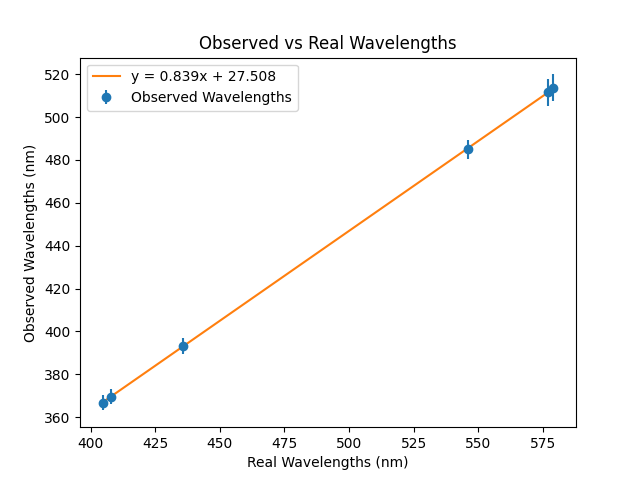
\includegraphics[width=0.8\textwidth]{Results/Sections/Part1/Part1_wavelength_observed_vs_expected.png}
    \caption{Observed vs expected wavelengths}
    \label{fig:Part1wave}
\end{figure}


\begin{figure}[H]
    \centering
    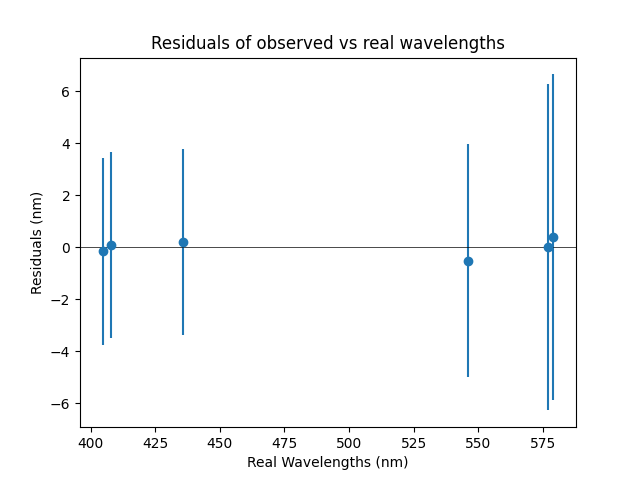
\includegraphics[width=0.8\textwidth]{Results/Sections/Part1/Part1_wavelength_observed_vs_expected_residuals.png}
    \caption{Observed vs expected wavelengths residuals}
    \label{fig:Part1waveU}
\end{figure}

line: 0.8387695642338823 ± 0.001864112875415517 x + 27.508082396595857 ± 0.9278156049052266
Chi squared: 1.087797528170102
Reduced chi squared: 0.2719493820425255



\begin{figure}[H]
    \centering
    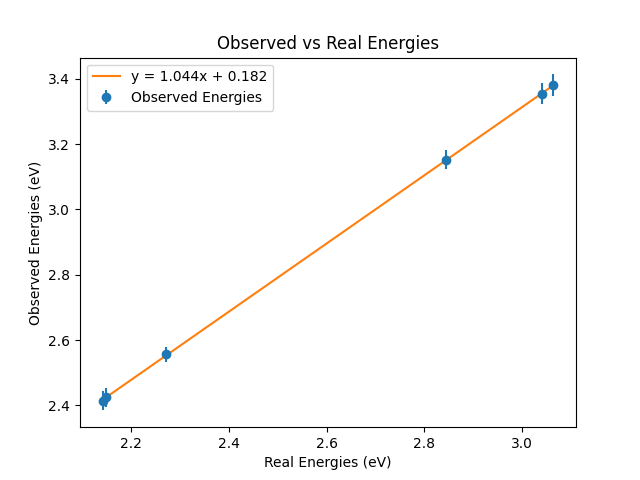
\includegraphics[width=0.8\textwidth]{Results/Sections/Part1/Part1_energy_observed_vs_expected.png}
    \caption{Observed vs expected energies}
    \label{fig:Part1energy}
\end{figure}

\begin{figure}
    \centering
    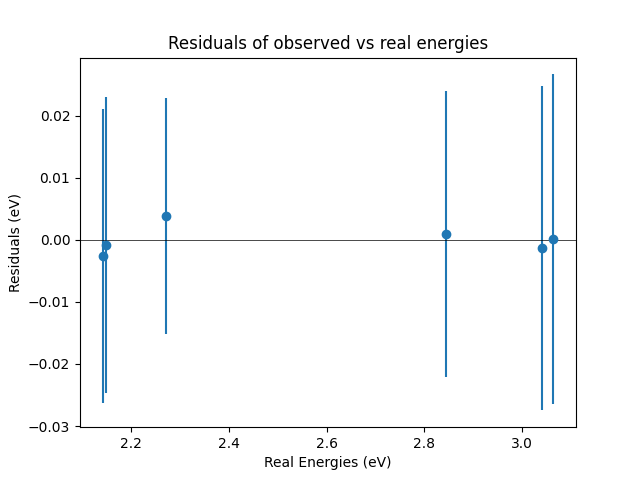
\includegraphics[width=0.8\textwidth]{Results/Sections/Part1/Part1_energy_observed_vs_expected_residuals.png}
    \caption{Observed vs expected energies residuals}
    \label{fig:Part1energyU}
\end{figure}

line: 1.0439270677118886 ± 0.0028012430069567747 x + 0.18182109169387295 ± 0.007329939614454457
Chi squared: 1.1027736664663765
Reduced chi squared: 0.27569341661659413